\documentclass{article}

\PassOptionsToPackage{numbers,compress}{natbib}
\usepackage[preprint]{neurips_2019}
% Keep the course template layout while removing its conference notice.
\makeatletter
\renewcommand{\@noticestring}{}
\makeatother
\usepackage[utf8]{inputenc}
\usepackage[T1]{fontenc}
\usepackage{hyperref}
\usepackage{url}
\usepackage{xurl}
\usepackage{booktabs}
\usepackage{amsfonts}
\usepackage{amsmath}
\usepackage{nicefrac}
\usepackage{microtype}
\usepackage{graphicx}
\graphicspath{{figures/}}

\title{Dreamer from Pixels: Midterm Baseline and Reproduction Plan}

\author{%
  Chevy Yang \\
  \texttt{chenyiy@andrew.cmu.edu}
  \And
  Zhiyuan Yang \\
  \texttt{dyang3@andrew.cmu.edu}
}

\begin{document}

\maketitle

\begin{center}
Team 25 \\
\textit{TA Mentor: Kangping Liu}
\end{center}

\begin{abstract}
We study visual control with Dreamer V1 in the DeepMind Control Suite. We use Julius Frost's PyTorch implementation, fix the source commit, and test the pipeline on \texttt{cartpole\_swingup} before extending to other tasks. The current baseline uses 64 x 64 RGB pixels, action repeat 2, one training seed, and 100,000 environment steps. A ten-update gate changed the world model, actor, and critic with finite diagnostics. In the longer run, the final policy reached mean episodic return 181.701 on ten fixed environment seeds, compared with 70.684 for the same model before training and 55.540 for a random policy. These results are initial evidence from one bounded run. We still need matched multi-seed runs and the two proposal experiments before drawing stronger conclusions.
\end{abstract}

\section{What We Want to Study}

Visual control requires an agent to learn both a useful representation and a policy from raw images. Dreamer addresses this problem with a learned latent dynamics model and policy improvement inside imagined trajectories. Our main goal is to reproduce and understand this Dreamer V1 pipeline from pixels. We start with \texttt{cartpole\_swingup}, then plan to evaluate \texttt{walker\_walk} and \texttt{ball\_in\_cup\_catch} after the baseline is stable.

We evaluate control with episodic return and learning curves. We do not use classification accuracy because the task is continuous control. We use a single training seed for the current pilot and keep the evaluation protocol separate from the training interaction. The current report is an initial baseline report, not a claim that we have matched the paper's full experimental study.

\section{Background and Related Work}

PlaNet introduced recurrent latent dynamics for planning from pixels \citep{hafner2019latent}. Dreamer follows the same general direction but replaces repeated online planning with value learning through latent imagination: it rolls the actor forward in the learned model and sends return gradients back through the imagined dynamics \citep{hafner2020dream}. We use Dreamer V1 as the baseline and cite PlaNet to explain the predecessor relationship; we do not combine their results or implementations.

We use Julius Frost's PyTorch implementation of Dreamer V1 at commit \texttt{ccea6ae4a397a94c328891bd78e81d52dd156cb6}, with the pinned \texttt{rlpyt} submodule at \texttt{f04f23db1eb7b5915d88401fca67869968a07a37} \citep{frost_dreamer_pytorch}. The DeepMind Control Suite provides the simulated continuous-control task and reward contract \citep{tassa2018dmcontrol}. We preserve the upstream MIT license and record our wrapper and measurement changes separately.
The original Google Research repository is retained as a historical Dreamer V1 software reference, not as a second implementation used in this run \citep{google_research_dreamer}.

\section{Method}

\subsection{Dreamer path}

The agent stores image sequences generated by real environment interaction. The world model encodes observations and infers a recurrent stochastic state. The actor and critic then operate on latent states imagined from replay states. Figure~\ref{fig:flow} summarizes the two paths.

\begin{figure}[t]
\centering
\setlength{\fboxsep}{5pt}
\begin{minipage}{0.44\linewidth}
\centering
\fbox{\parbox[c][0.55in][c]{0.9\linewidth}{\centering\textbf{Real interaction}\\
pixels $o_t$ $\rightarrow$ encoder/RSSM posterior $\rightarrow$ action $a_t$ $\rightarrow$ DMC step}}

\vspace{3pt}
\fbox{\parbox[c][0.42in][c]{0.9\linewidth}{\centering replay sequence\\
pixel preprocessing and temporal storage}}
\end{minipage}
\hspace{0.04\linewidth}
\begin{minipage}{0.44\linewidth}
\centering
\fbox{\parbox[c][0.55in][c]{0.9\linewidth}{\centering\textbf{Latent imagination}\\
replay state $\rightarrow$ RSSM prior rollout $\rightarrow$ actor + critic}}

\vspace{3pt}
\fbox{\parbox[c][0.42in][c]{0.9\linewidth}{\centering imagined returns\\
actor gradients through frozen dynamics}}
\end{minipage}
\caption{Our simplified Dreamer data flow. Real interaction supplies image sequences to replay. Training starts from replay states and uses the learned RSSM for latent imagination; the critic supplies return targets and actor gradients pass through the imagined dynamics.}
\label{fig:flow}
\end{figure}

The environment wrapper renders camera 0 as a 64 x 64 RGB image and stores it as a uint8 tensor in channel-first format. Before the encoder, the implementation converts pixels from $[0,255]$ to $[-0.5,0.5]$. One action is repeated for two underlying environment steps. Thus, 50,000 policy decisions correspond to 100,000 environment steps. Episodes contain 500 decisions, or 1,000 environment steps. The replay buffer stores temporal sequences, and the training batch has 16 sequences of length 50.

\subsection{Objectives used in this run}

The world model learns an observation reconstruction distribution, a reward distribution, and an RSSM prior/posterior agreement term. The implementation also supports a continuation-probability head, but our formal run uses \texttt{use\_pcont=False}. Therefore, the continuation head is not constructed, its loss is not included in the world-model objective, and the imagined-return calculation uses the fixed discount factor instead. The logged \texttt{pcont\_loss} field is a zero placeholder when this option is disabled; it is not evidence that a continuation loss was trained.

The actor is trained on returns imagined from posterior states, while the critic predicts those imagined returns. The main checks for the debug gate were finite losses and gradients, nonzero changes to all three parameter groups, and loading the saved model in a new process. We do not claim full optimizer/replay/environment-state continuation from the exported checkpoint.

\begin{table}[t]
\caption{Effective configuration of the 100k-environment-step run.}
\centering\small
\begin{tabular}{ll}
\toprule
Task / observation & cartpole\_swingup, camera 0, 64 x 64 RGB \\
Training seed & 0 \\
Decision / environment budget & 50,000 / 100,000 \\
Action repeat / episode limit & 2 / 500 decisions (1,000 env steps) \\
Prefill & 1,000 decisions (2,000 env steps) \\
Training schedule & every 1,000 decisions, 100 updates \\
Batch size / length & 16 / 50 \\
Replay capacity & 60,000 decision transitions \\
Precision / \texttt{use\_pcont} & 32-bit / False \\
Evaluation environment seeds & 1000--1009 \\
\bottomrule
\end{tabular}
\end{table}

\section{Baseline and Experimental Iteration}

We first tried the historical TensorFlow route, but the available Python/Keras environment exposed old API and MuJoCo dependency failures. We then used the pinned PyTorch source in the already working Kaggle PyTorch environment. A fresh child process passed the CPU \texttt{dm-control} import/reset probe, and the GPU path passed CUDA, EGL pixel rendering, and the short Dreamer update gate. We reused the validated \texttt{dm-control --no-deps} route rather than changing the algorithm to fit a new dependency stack. These environment changes matter for reproducibility, but they are not separate scientific experiments.

Before the longer run, we corrected an intermediate configuration with \texttt{train\_every=1} and \texttt{train\_steps=8}; the formal run restored the upstream-style schedule of 1,000 decisions and 100 updates. We also increased replay capacity from the short pilot's 1,060 decision transitions to 60,000. The initial comparison is a snapshot of the formal training model after prefill and before its first optimizer update, not a separately initialized policy.

\begin{table}[t]
\caption{Two pilot configurations. Budget, replay, and initial-checkpoint handling changed together; this is not a one-factor ablation.}
\centering\small
\begin{tabular}{lcc}
\toprule
 & 6k pilot & 100k run \\
\midrule
Decision / environment steps & 3,000 / 6,000 & 50,000 / 100,000 \\
Replay capacity (decision transitions) & 1,060 & 60,000 \\
Batch size x length & 16 x 50 & 16 x 50 \\
Train every / updates & 1,000 / 100 & 1,000 / 100 \\
Initial comparison & short-run snapshot & formal pre-update snapshot \\
Final Dreamer mean return & 115.463 & 181.701 \\
\bottomrule
\end{tabular}
\end{table}

\section{Results}

The ten-update gate changed the world model, actor, and critic by maximum absolute parameter differences of 0.011696, 0.000710, and 0.000771. The formal run completed 50,000 decisions, 100,000 environment steps, and 4,900 optimizer updates. The raw checkpoint, metrics, progress file, configuration, and evaluation CSV were downloaded and checked.

We evaluated three policies on the same ten environment seeds, 1000--1009. Each policy therefore has ten episodes; these are not ten training seeds. Training seed 0 is the only training seed in this report. The reported $\pm$ values are sample standard deviations across evaluation episodes. We controlled the environment seed, but we do not claim that every source of evaluation randomness was fixed.

\begin{table}[t]
\caption{Evaluation on ten episodes for each policy, using environment seeds 1000--1009.}
\label{tab:returns}
\centering\small
\begin{tabular}{lrr}
\toprule
Policy & Mean return & Episode sample std. \\
\midrule
Random & 55.5404 & 42.5973 \\
Training-initial & 70.6835 & 3.1504 \\
Final Dreamer & 181.7011 & 27.5705 \\
\bottomrule
\end{tabular}
\end{table}

The final mean return is higher than the training-initial snapshot and the random control in this pilot. The theoretical maximum episodic return is 1,000, so 181.7 is still a limited absolute score. Return is not success rate. The final policy also has visible episode-to-episode variation, so the mean alone is not a complete description.

Figure~\ref{fig:results} shows two different measurements. The left panel is the training \texttt{ReturnAverage} from rlpyt: an average over up to the 100 most recently completed training episodes at each logging point. It is a windowed training diagnostic, not an evaluation learning curve. It rises from roughly the low 70s near the prefill boundary to roughly 120 near the end, with fluctuations after the early increase. Training uses exploration noise, so this curve should not be read as the same quantity as the final evaluation table. The right panel shows all raw evaluation episode returns as points, together with the mean and the sample standard deviation.

\begin{figure}[t]
\centering
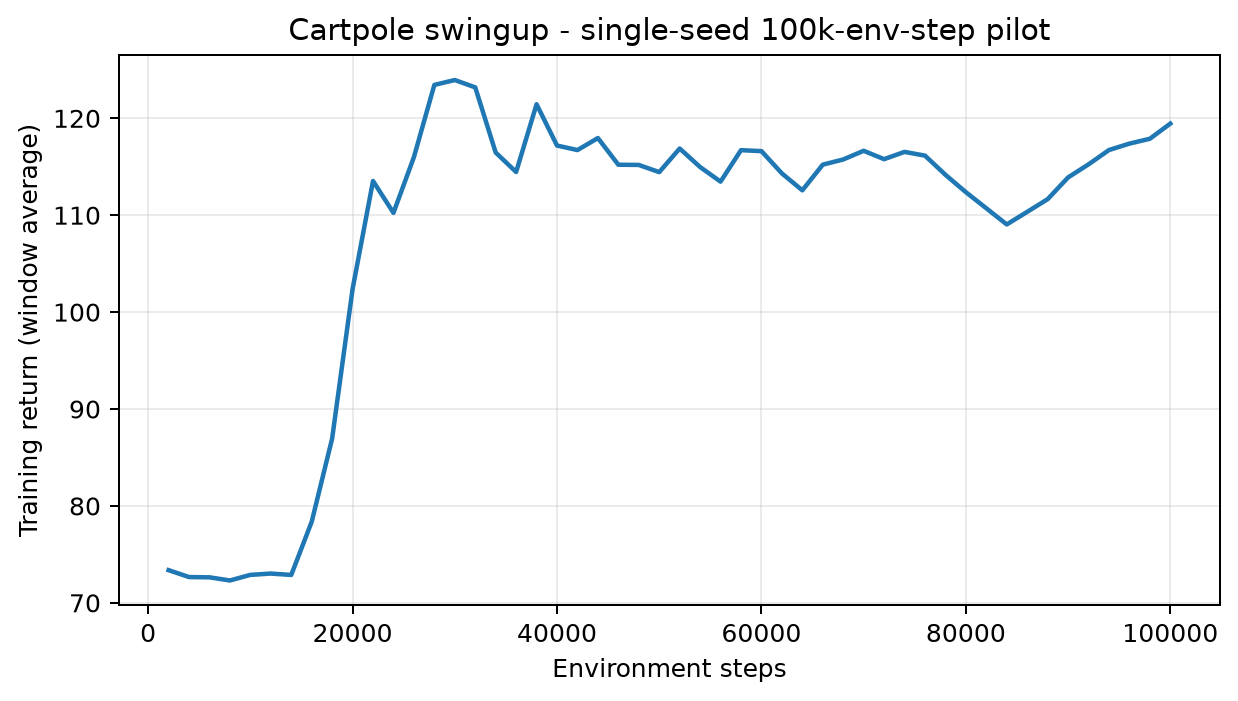
\includegraphics[width=0.49\linewidth]{training_return_vs_env_steps.png}
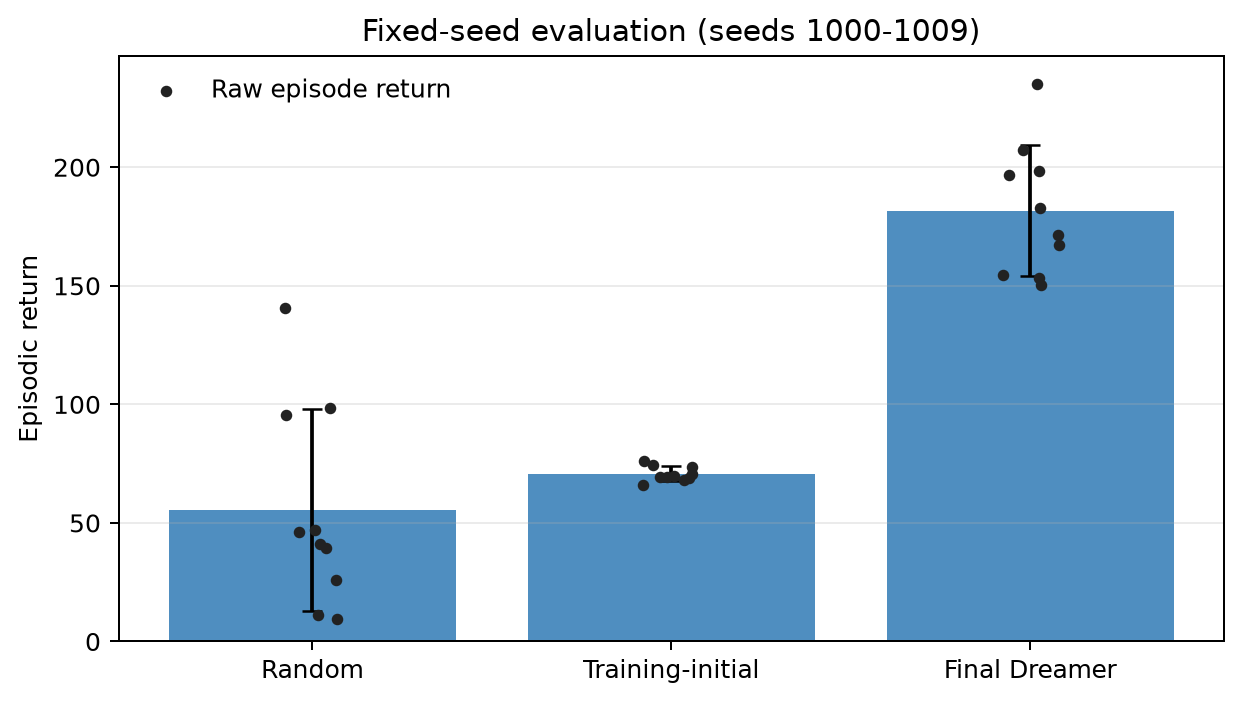
\includegraphics[width=0.49\linewidth]{evaluation_comparison.png}
\caption{Left: rlpyt training-return window average versus environment steps. The x-axis is environment steps; the underlying log records decision steps and action repeat is 2. Right: fixed-seed evaluation; black points are the ten raw episode returns for each policy and error bars are the sample standard deviation across those ten episodes.}
\label{fig:results}
\end{figure}

\section{Limitations and Future Work}

The current evidence comes from one task, one training seed, and a bounded budget. We do not claim statistical significance, stable task mastery, or paper-level performance. The plots do not identify a specific failure behavior, and we do not infer that low returns are caused by a particular code bug or only by insufficient training. The checkpoint was loaded for evaluation, but full restoration of optimizer, replay, and environment state remains untested.

Our next steps follow the proposal. First, we will inspect evaluation videos, the fixed-seed protocol, and the training curve to decide whether the baseline should run longer. Second, we will add training seeds 1 and 2 with the same budget and configuration. Third, we will run matched-budget sensitivity experiments for the proposal's two directions: (i) imagination horizons such as 5, 15, and 30, which are candidate settings and have not been executed; and (ii) a 4-pixel random-shift image augmentation. For the random-shift study, we will specify padding and crop behavior before implementation, keep the transform consistent within each replay sequence, and document how the encoder input and decoder reconstruction target are transformed. We will not assume that augmentation improves performance.

\section{Conclusion}

We now have a working Dreamer V1 training and evaluation pipeline for pixel-based \texttt{cartpole\_swingup}. The formal run changed all three learned modules and produced a higher final mean return than its pre-update snapshot under the same ten evaluation environment seeds. This is useful baseline evidence, but replication still requires matched additional training seeds, protocol checks, and the two proposal experiments.

\section*{Team Contributions (Pending Confirmation)}

Chevy Yang and Zhiyuan Yang both contributed to the seed-0 Dreamer V1 baseline, including experiment setup, execution, and review of the resulting evidence. The report treats this as one shared training run, not as independent training seeds. The finer division of implementation, artifact preparation, and analysis will be finalized after the team confirms the remaining details.

\section*{GitHub}

Project repository: \url{https://github.com/DDaniel-code/dreamer-pixels}. The repository records the selected source commit, configuration differences, raw-artifact manifest, and report materials.

\begingroup
\small
\bibliographystyle{plainnat}
\bibliography{dreamer_pixels_midterm_report}
\endgroup

\end{document}
